\section{Methods}
\section{Refinement}

\subsection{Occupancy group definition}\label{sup:occupancy}
Script written for the definition of occupancy groups, creating a file passed to Refmac for occupancy refinement. The script parses PDB and detects residues with alternate conformations, water molecules and ions. 

It runs as follow: \mintinline{bash}{write_occ_inp.sh > ref.inp}

\begin{minted}[breaklines=True]{bash}
#!/bin/bash 
if [ -z "${1}" ]  #1st param of the function
then
    read -p "Enter path to coordinate file: " model
else
    model="${1}"
fi
echo "fetching coordinates from $model"
rm ref.inp
touch ref.inp
#looping over the lines of the reslist
group_id=1
#grep all residues that have altconfs
grep "^ATOM" $model | cut -c 17-26 | grep "[A-Z][A-Z][A-Z][A-Z]" | cut -c 2-10 | sort -u | awk '{print $1,$3}' > listres
grep "^HETATM" $model | cut -c 17-26 | grep "[A-Z][A-Z][A-Z][A-Z]" | awk -F "" '{OFS="";print $2,$3,$4," ",$7,$8,$9,$10}' | sort -u >> listres 
#grep ions
grep "^HETATM" $model | grep -v "HOH" | cut -c 17-26 | grep -v "[A-Z][A-Z][A-Z][A-Z]" | awk -F "" '{OFS="";print $2,$3,$4," ",$7,$8,$9,$10}' | sort -u > tmp
awk -F "\t" 'NR==FNR{a[$1]=$1} !($1 in a) && (NR>FNR) {print $0}' listres tmp > listres_ions


while IFS='' read -r LINE || [ -n "${LINE}" ]; do   
   echo "${LINE}" > tmp
   resname=`awk '{print $1}' tmp`
   resid=`awk '{print $2}' tmp`
   #add a loop through the alphabet to categorise all altconf
   for alt in {A..Z}
   do
   #no need to run through the whole alphabet, we only need the letters corresponding to the present altconfs in the model
   is_the_alt_there=`grep "$alt$resname" $model | grep "$resid"`
   if [[ ! -z $is_the_alt_there ]]
   then
   #better safe than sorry
   echo "processing $alt$resname $resid group $group_id"
   #heavy lifting line
   if [[ "$resid" -gt 999 ]] #some duct tape to fix the annoying column based pdb format. If resid is 4 char wide it's glued to the chain and it needs to be splaced
   then
   grep "$resname" $model | grep -v "LINKR" |grep "$resid" |grep "$alt$resname" | sed "s/$alt$resname/ $resname/g" | sed "s/$resid/ $resid/g" | head -n1 |awk -v altconf="$alt" -v groupid="$group_id" '{print "occupancy", "group", "id", groupid ,"chain", $5, "residue", $6, "alt", altconf}' >> ref.inp
   else #if not, then nothing to do and we can grep as is 
   grep "$resname" $model | grep -v "LINKR" |grep "$resid" |grep "$alt$resname" | sed "s/$alt$resname/ $resname/g" | head -n1 | awk -v altconf="$alt" -v groupid="$group_id" '{print "occupancy", "group", "id", groupid ,"chain", $5, "residue", $6, "alt", altconf}' >> ref.inp
   fi
   #one group id is done, we can increment the counter and store the name of the group to write the complete instruction
   linked_groups=`echo "$linked_groups $group_id"`
   let group_id=group_id+1
   fi
   done
   echo "ensemble $linked_groups"
   echo "occupancy group alts complete$linked_groups" >> ref.inp
   #then reset the storage (but not the counter)
   linked_groups=
done < listres
while IFS='' read -r LINE || [ -n "${LINE}" ]; do   
   echo "${LINE}" > tmp
   resname=`awk '{print $1}' tmp`
   resid=`awk '{print $2}' tmp`
   echo "processing $resname $resid group $group_id"
   #heavy lifting line
   chain=`grep "$resname" $model | grep 'HETATM' | awk -F "" '{OFS="";print $22}' | sort -u`
   echo "occupancy group id $group_id chain $chain residue $resid" >> ref.inp  
   echo "occupancy group alts incomplete $group_id" >> ref.inp
   echo "ensemble $group_id"
   let group_id=group_id+1
done < listres_ions

echo "occupancy refine ncyc 5"  >> ref.inp
echo "occupancy" >> ref.inp
echo "refine" >> ref.inp
echo "eor" >> ref.inp
\end{minted}

\section{Supplementary materials - Twist-Cerulean, a pH-sensitive fluorescent protein}\label{sup:T-Cer}

\begin{figure}
    \centering
    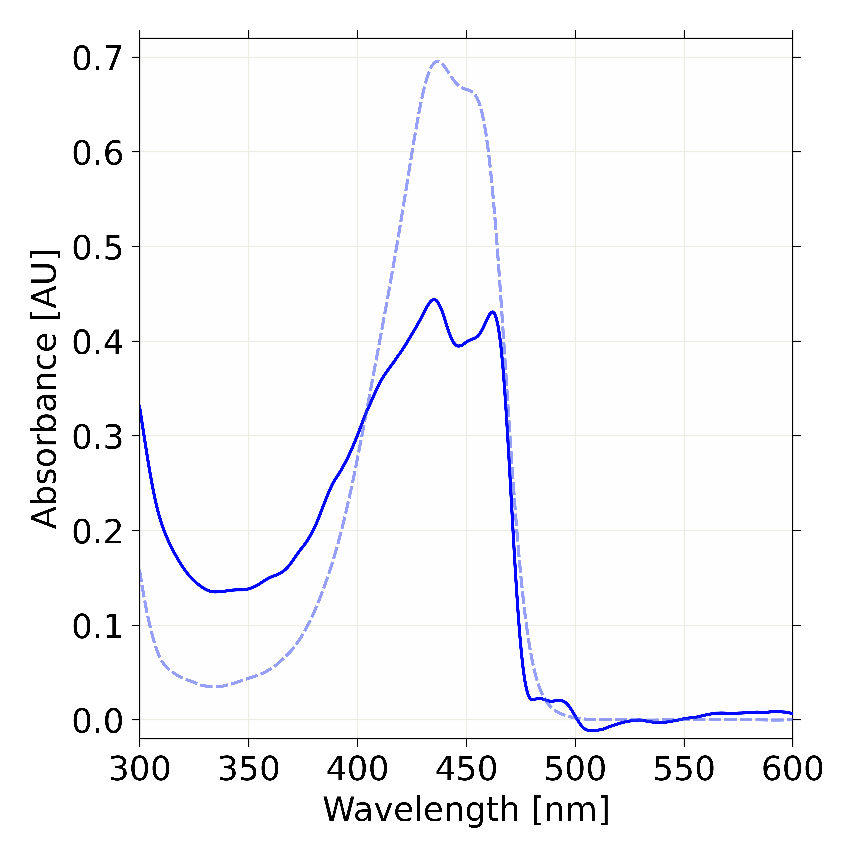
\includegraphics{images/T-Cer/T-Cer_ic_pH8.pdf}
    \caption{ In solution, at room temperature (dashed line) and \textit{in crystallo} absorption spectra (full line) featuring the same maximum of absorbance around 438 nm. Of note, the 450 nm shoulder of the in-solution spectrum becomes a peak in the \textit{in crystallo} spectrum, and the \textit{in crystallo} spectrum features an additional shoulder around 410 nm and one around 380 nm. Finally, the dip in absorbance at 510 nm in the \textit{in crystallo} spectrum is caused by fluorescence (see Chapter \ref{chap:toolbox}).}
    \label{supfig:pH8_spec}
\end{figure}

\subsection{pH stability of T-Cer}

\begin{figure}
    \centering
    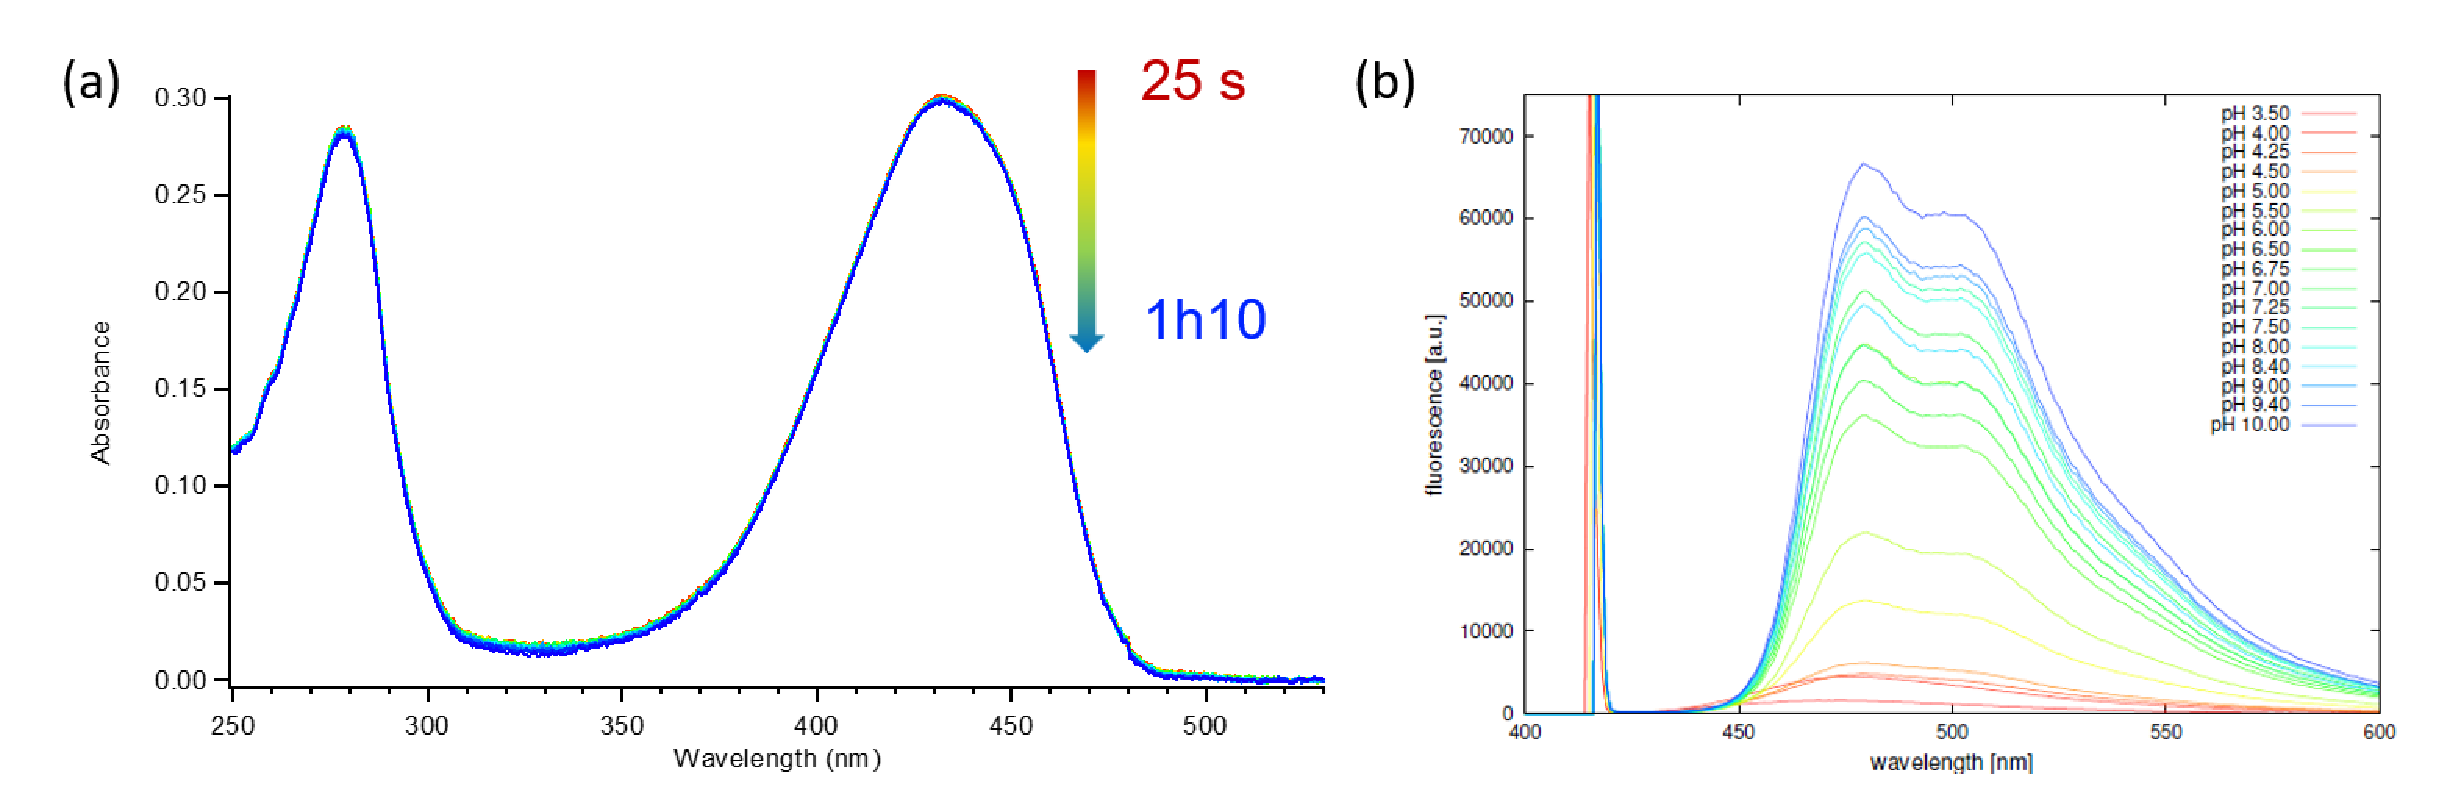
\includegraphics{images/T-Cer/suppfig_fluo_pHjumplong.pdf}
    \caption{(a) Follow-up of the time-resolved spectroscopy experiment in solution, on the second (red) to hour (blue) time-scale, showing that the peak of T-Cer remains stable after its initial fast blue-shift. (b) Fluorescence spectrum of T-Cer over pH, from neutral (blue) to acidic (red) pH. Data recorded and figure prepared by David von Stetten}
    \label{supfig:Fluo_T-Cer}
\end{figure}

\section{First time-resolved experiments: tape drive on P11}\label{sec:P11-1}

Proposals for several TR-SSX experiments studying the conformation switch of T-Cer's chromophore triggered by a pH drop were submitted at the very beginning of this PhD. Due to the COVID19 health crisis, the first experiment happened remotely in 2021, on beamline P11, at Petra III. A second beamtime on beamline P11 happened in person, in December 2021.   
P11 can accommodate a TR-SSX setup, called the CFEL tape drive \parencite{beyerleinMixanddiffuseSerialSynchrotron2017,zielinskiRapidEfficientRoomtemperature2022}. This particular setup is suited for time-delays from the 100s of ms to the tens of seconds and allows fast mixing.

\subsection{First remote beamtime}\label{sec:P11_1}

In June 2021, the first TR-SX experiment on T-Cer took place at P11 (Petra III). Due to the COVID19 health crisis, the experiment was done remotely. The protein crystals, as well as all pH buffers, precipitants, and crystal seeds were sent to Petra III ahead of time and the P11 team gracefully accepted to set up the experiment and record a series of time points previously fixed. To induce a pH drop in T-Cer crystals, they were mixed with a lower pH mother liquor solution (described in Section \ref{sec:presenting_tpd_P11}). Beamline P11 is a standard high-throughput MX beamline, with a focused beam size of \(4 \times 9 \mu m\), and a flux of \(10^{13}\) photons/s, at an energy level of 12 keV. It is operated by the Deutsches Elektronen-SYnchrotron (DESY).

The experimental plan was drafted with the results of the in-solution time-resolved absorption spectroscopy experiment in mind (see Section \ref{sec:prior_T-Cer}), with time points across the ms regime. A ground-state (neutral pH T-Cer crystals, no mixing) dataset was recorded before the mixing experiment, and after, for comparison.

The data collected during this beam-time was processed by members of the Chapman group (details of the processing are available in Section \ref{sec:T-Cer_methods}). The unit cell parameters of both room temperature neutral pH (ground-state) datasets (see Table \ref{tab:P11_tpd1}) were identical. The C axes of these room temperature neutral pH datasets (Table \ref{tab:P11_tpd1}) are longer than those of the cryogenic temperature neutral pH dataset (see Table \ref{tab:structure-list}) by 1 \AA. Such an expansion is well documented when comparing cryogenic (100 K) and room temperature (220 K) datasets. 

No meaningful differences could be identified between the two ground states, either by visual inspection or isomorphous difference map. In ideal conditions (ground, no mixing), the T-Cer crystals diffracted to 1.9 \AA. All key amino acids of the chromophore pocket, as well as the chromophore itself, were in the same conformation as in the cryogenic dataset (See Fig. \ref{fig:tpd1} (a) for the 220K dataset, and Fig. \ref{fig:T-Cer_pH8vs4}  (a) for the 100K dataset).  All datasets in the time series also diffracted to 1.9 \AA, despite containing significantly fewer indexed frames. This is somewhat expected because (1) the detector to sample distance was set so that the edge of the detector was at 2 \AA, and (2) all datasets are largely above the advised number of indexed diffraction patterns for a dataset \footnote{The resolution of an SSX dataset, as well as all its data-quality metrics, are tightly linked to the number of indexed diffraction pattern used to make it, but only up to a certain point. There is no clear-cut answer on a reasonable number of frames to get a complete serial-crystallography dataset, a survey of the literature suggests 10 000 indexed diffraction patterns to be a good estimation \parencite{pearsonSerialSynchrotronCrystallography2020, zielinskiRapidEfficientRoomtemperature2022}. Of note, in order to push resolution to its absolute limits, a much larger number of frames are needed. Such was the case for the data collected at SwissFEL for \cite{maestre-reynaVisualizingDNARepair2023a}, for instance.} and the edge of the detector was set to 2 \AA.

Unfortunately, there was no meaningful difference between any of the time points collected (see Table \ref{tab:P11_tpd1}) and the merged ground dataset (see Fig. \ref{fig:tpd1} (a) vs (b)), whether assessed by surveying a \(Fo _{light} - Fo_{dark}\) isomorphous difference map, or the \(F_{obs} - F_{calc}\) map produced by refining a dataset against the ground state model. The density on V150 remains well defined through the first second after mixing, as well as E222 and S205, as visible in the electron density of the last time point collected (760 ms, Fig. \ref{fig:tpd1}). Accordingly, the unit cells of all time points are identical to that of the ground states (Table \ref{tab:P11_tpd1}), while the acidic pH cryogenic datasets had 'shrunk' unit cell constants (Table \ref{tab:structure-list}).

\begin{figure}[H] %bt!]
    \centering
        \noindent 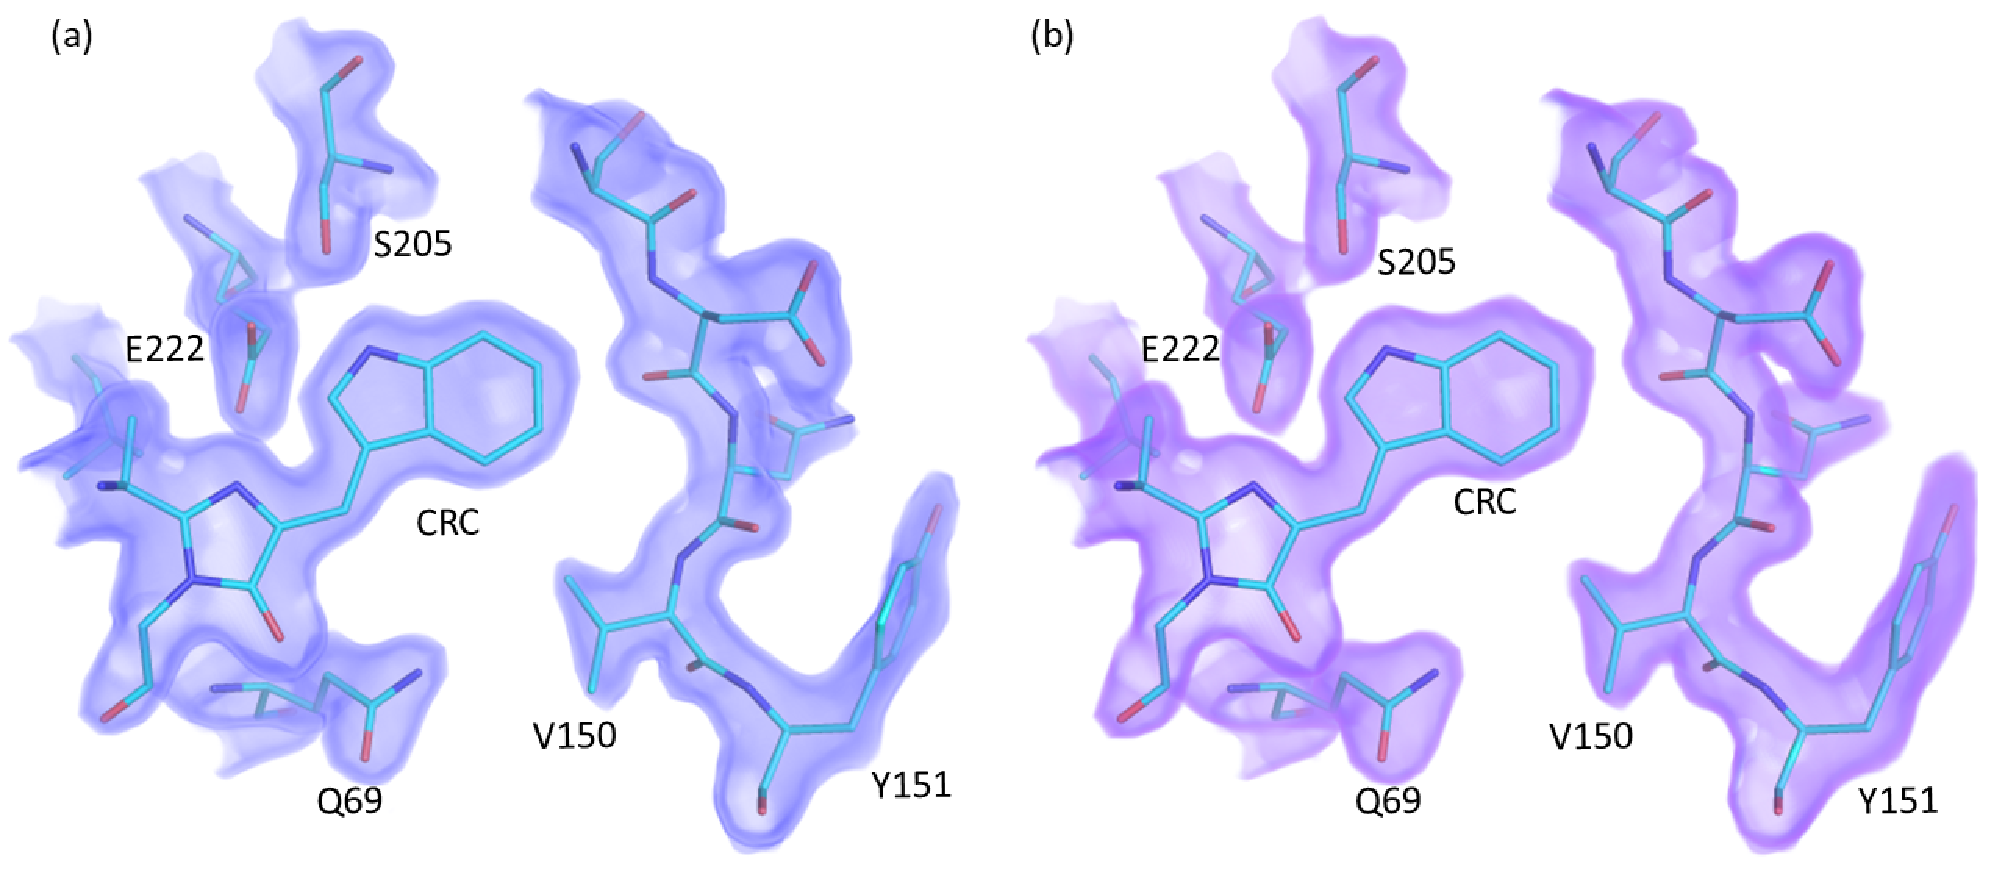
\includegraphics[width=\textwidth]{images/T-Cer/P11_1_volumes.pdf}
    \hfill
    \caption{Electron density maps (2\(F_{obs} - F_{calc}\)) of the chromophore pocket of T-Cer (a) at neutral pH in its ground state (b) 760 ms after mixing has occurred. Both maps are contoured at 1 r.m.s.d. displayed 1.4 \AA  around the selected amino acids. Both electron density maps are almost identical, with well-defined electron density on V250, and single conformations of S205 and E222. The H-bond between E22 and S205 is visible.}
    \label{fig:tpd1}
\end{figure}
\begin{table}[H]
    \centering
    \begin{tabular}{| m{1.5cm} | m{1.2cm} | m{1.5cm} | m{1.5cm} | m{1.5cm} | m{1cm} | m{1.2cm} | m{1.2cm} |}
        \hline
        Time after pH mix (ms) & Volume used & num frames & hits & indexed crystals & hit rate & indexing rate & unit cell C-axis\\
        \hline
        ground & 498 \textmu l & 4.85E+05 & 7.47E+04 & 4.99E+04 & 0.15 & 0.56 & 70.67\\
        \hline
        ground & 83.3 \textmu l & 2.00E+05 & 1.95E+05 & 1.95E+05 & 0.97 & 0.69 & 70.68\\
        \hline
        40 & 83.3 \textmu l & 2.00E+05 & 1.38E+05 & 5.56E+04 & 0.69 & 0.34 & 70.6\\
        \hline
        67 & 83.3 \textmu l & 2.00E+05 & 1.79E+05 & 1.39E+05 & 0.89 & 0.57 & 70.73\\
        \hline
        120 & 83.3 \textmu l & 2.00E+05 & 1.98E+05 & 1.83E+05 & 0.99 & 0.64 & 70.72\\
        \hline
        320 & 83.3 \textmu l & 2.00E+05 & 1.72E+05 & 1.04E+05 & 0.86 & 0.46 & 70.66\\
        \hline
        760 & 83.3 \textmu l & 2.00E+05 & 1.97E+05 & 2.58E+05 & 0.99 & 0.79 & 70.85\\
        \hline
    \end{tabular}
    \caption{Collection logs from the tape drive experiment on P11}
    \label{tab:P11_tpd1}
\end{table}

This is likely because the time points chosen based on the time-resolved in solution spectroscopy experiment were too short to allow both a successful mixing, and any protein movements to happen, and because the pH drop was not drastic enough. During the experiment, the flow of acidic pH solution was twice as high as that of the crystal sample suspension, the resulting pH after mixing is of \textasciitilde 5.5, which might not be enough to trigger the conformation change, since at pH 6.0 in solution, the spectrum of T-Cer has lost its double-peaked nature, but has not blue-shifted yet (Fig. \ref{fig:pH_TRspectroinsolution}). For future experiments, it was decided to use pure 1 M pH buffer as the acidic pH solution, so that the mixed solution would be approximately at pH 4.0.

Despite the absence of protein movements, this experiment was a successful proof of principle since good quality datasets of T-Cer were collected. Further, the amount of sample consumed to obtain a very good quality dataset was moderate with less than 1 ml of sample used in total, 83 \textmu l for a dataset (Table \ref{tab:P11_tpd1}) out of 3 ml of sample sent and 3 ml of sample crystallised on-site at PETRA III).

\subsection{New space group for T-Cer-s}\label{sec:newspacegroup}

T-Cer-s was first crystallised using the same crystallisation condition at neutral pH as T-Cer (Section \ref{sec:T-Cer_methods}). Interestingly, crystals only grew at 14 \% PEG, and as a pile-up of plates (Fig. \ref{fig:T-Cer-fristcryst} (d)) diffracting to moderate (1.9 \AA, vs sub \AA\ for standard crystals of T-Cer bigger than 100 \textmu m) resolution, but with a novel, less dense crystal packing (See a comparison of both packings in Fig. \ref{fig:T-Cer-fristcryst} (a) vs (b)). The datasets of T-Cer-s indexed in space group 20 (C 2 2 2\textsubscript{1}), with unit cell axis lengths of (61.09\AA, 94.15\AA, 117.77\AA). However, crystals grown in the low pH condition for T-Cer (Section \ref{sec:ageing}) had the expected packing of crystals of T-Cer in space group 19, with short unit cell constants (Table \ref{tab:structure-list}).

The packing of T-Cer-s is interestingly less denser than that of T-Cer crystals (Fig. \ref{fig:T-Cer-fristcryst} (a) and (b)). It was thus explored by soaking experiments, but crystals only survived the soak for less than 2 s, at which point the lattice parameters had not changed and the chromophore pocket was still the same (Fig. \ref{fig:T-Cer-fristcryst} (c)). 

\begin{figure}[H] %bt!]
    \centering
        \noindent 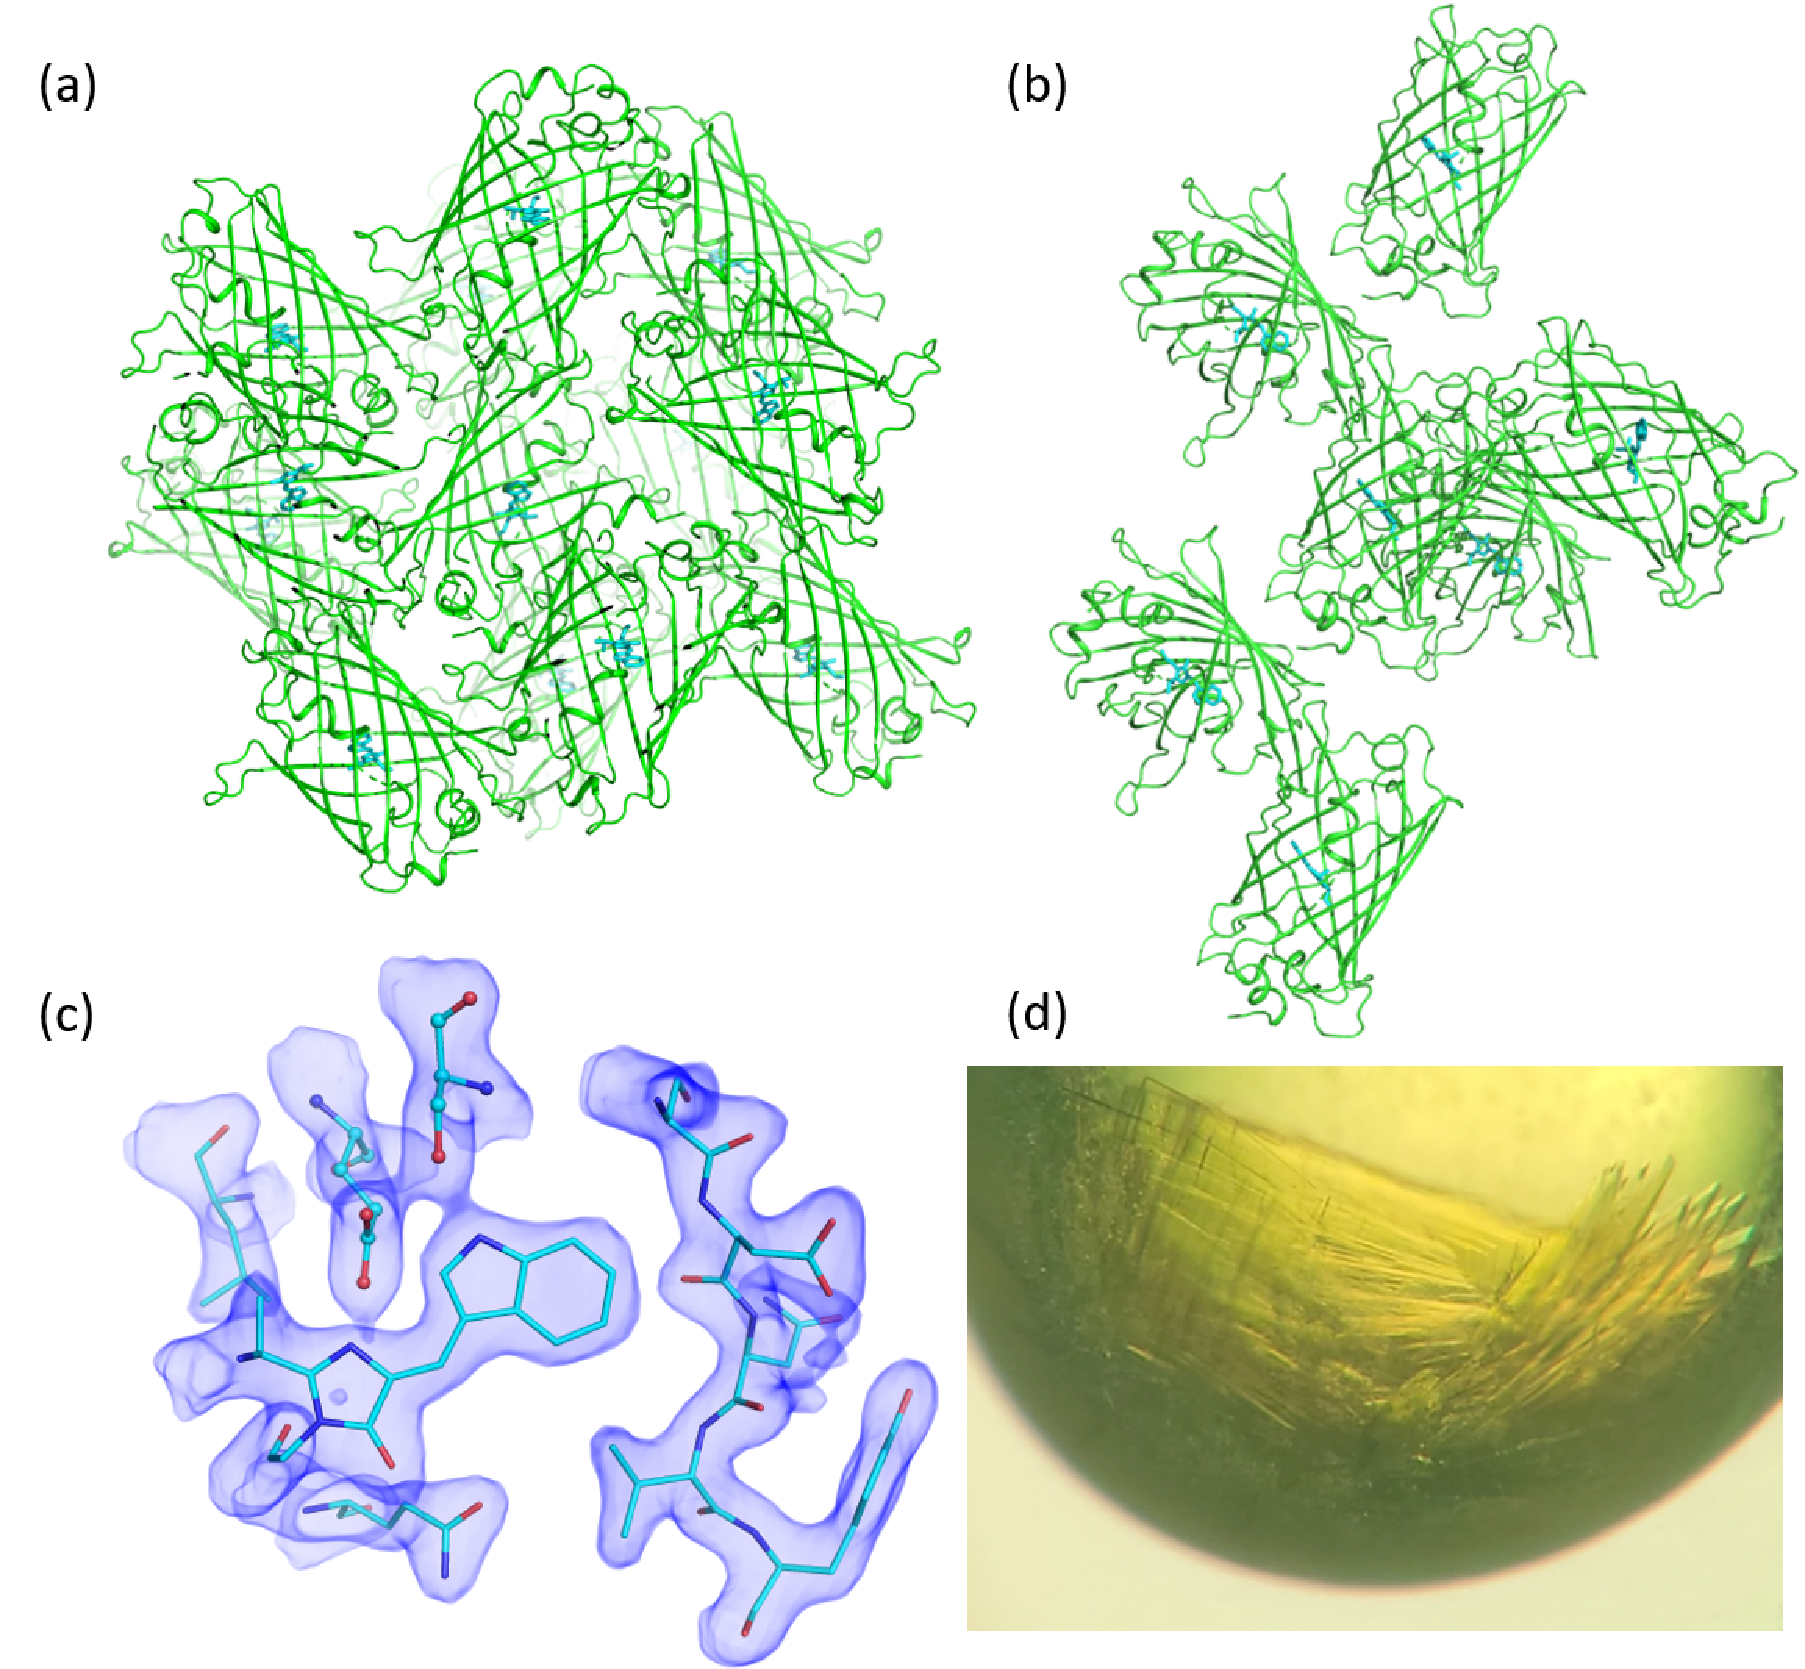
\includegraphics[width=\textwidth]{images/T-Cer/T-Cer-s_firstcrystals.pdf}
    \hfill
    \caption{Comparison of the packing of T-Cer P 2\textsubscript{1} 2\textsubscript{1} 2\textsubscript{1} (a) and T-Cer-s C 2 2 2\textsubscript{1} (b) crystal packing obtained by displaying all symmetry relatives located at 10 \AA of the central monomer.  The packing of T-Cer-s crystals is significantly looser. 
    Characterisation of the first T-Cer-s. (c) Electron density map (2\(F_{obs} - F_{calc}\), 2.5 \AA resolution) of the a T-Cer-s crystal soaked in 1 M pH 4.0 sodium citrate buffer. E222 is still H-bonded to S205. The electron density on all amino acids of the 7\textsuperscript{th} strand are well defined. (d) Plate shaped crystals of T-Cer-s in the C 2 2 2\textsubscript{1} crystal form}\label{fig:T-Cer-fristcryst}
\end{figure}

The C 2 2 2\textsubscript{1} crystal form of T-Cer-s diffracts to moderate resolutions and form plates stacked onto each other (Fig. \ref{fig:T-Cer-fristcryst} (d)). Despite its looser packing (Fig. \ref{fig:T-Cer-fristcryst} (c)), isomerization does not seem to happen faster in this crystal form.  Crystallising the P 2\textsubscript{1} 2\textsubscript{1} 2\textsubscript{1} crystal form was important to increase data quality. 

Several proteins have been crystallised from crystal seeds of their homolog or variants \parencite{bergforsSeedsCrystals2003}. The crystallisation condition which yielded the first, C 2 2 2\textsubscript{1} crystals of T-Cer-s were replicated, and supplemented with a 1/1000 000 dilution of a micro-seed suspension of T-Cer (See Section \ref{sec:microcrystallisation} for the protocol used to prepare a seed suspension).  Crystals of T-Cer-s in P 2\textsubscript{1} 2\textsubscript{1} 2\textsubscript{1} grew after two days, with the same shape (Elongated rectangular prisms similar to those visible on the second panel of Fig. \ref{fig:Crystallisation_T-Cer}) as T-Cer crystals. 


\section{Supplementary materials - The early steps in signalling from a bifunctional cryptochrome, traced by TR-SFX and TR-\textit{ic}OS}\label{sup:CraCRY_TR-SFX_1_sup}
\section{Supplementary materials - Visualising the rise of the signalling state of a cryptochrome with the TR-SOX method}




\begin{figure}[H]
  \centering
  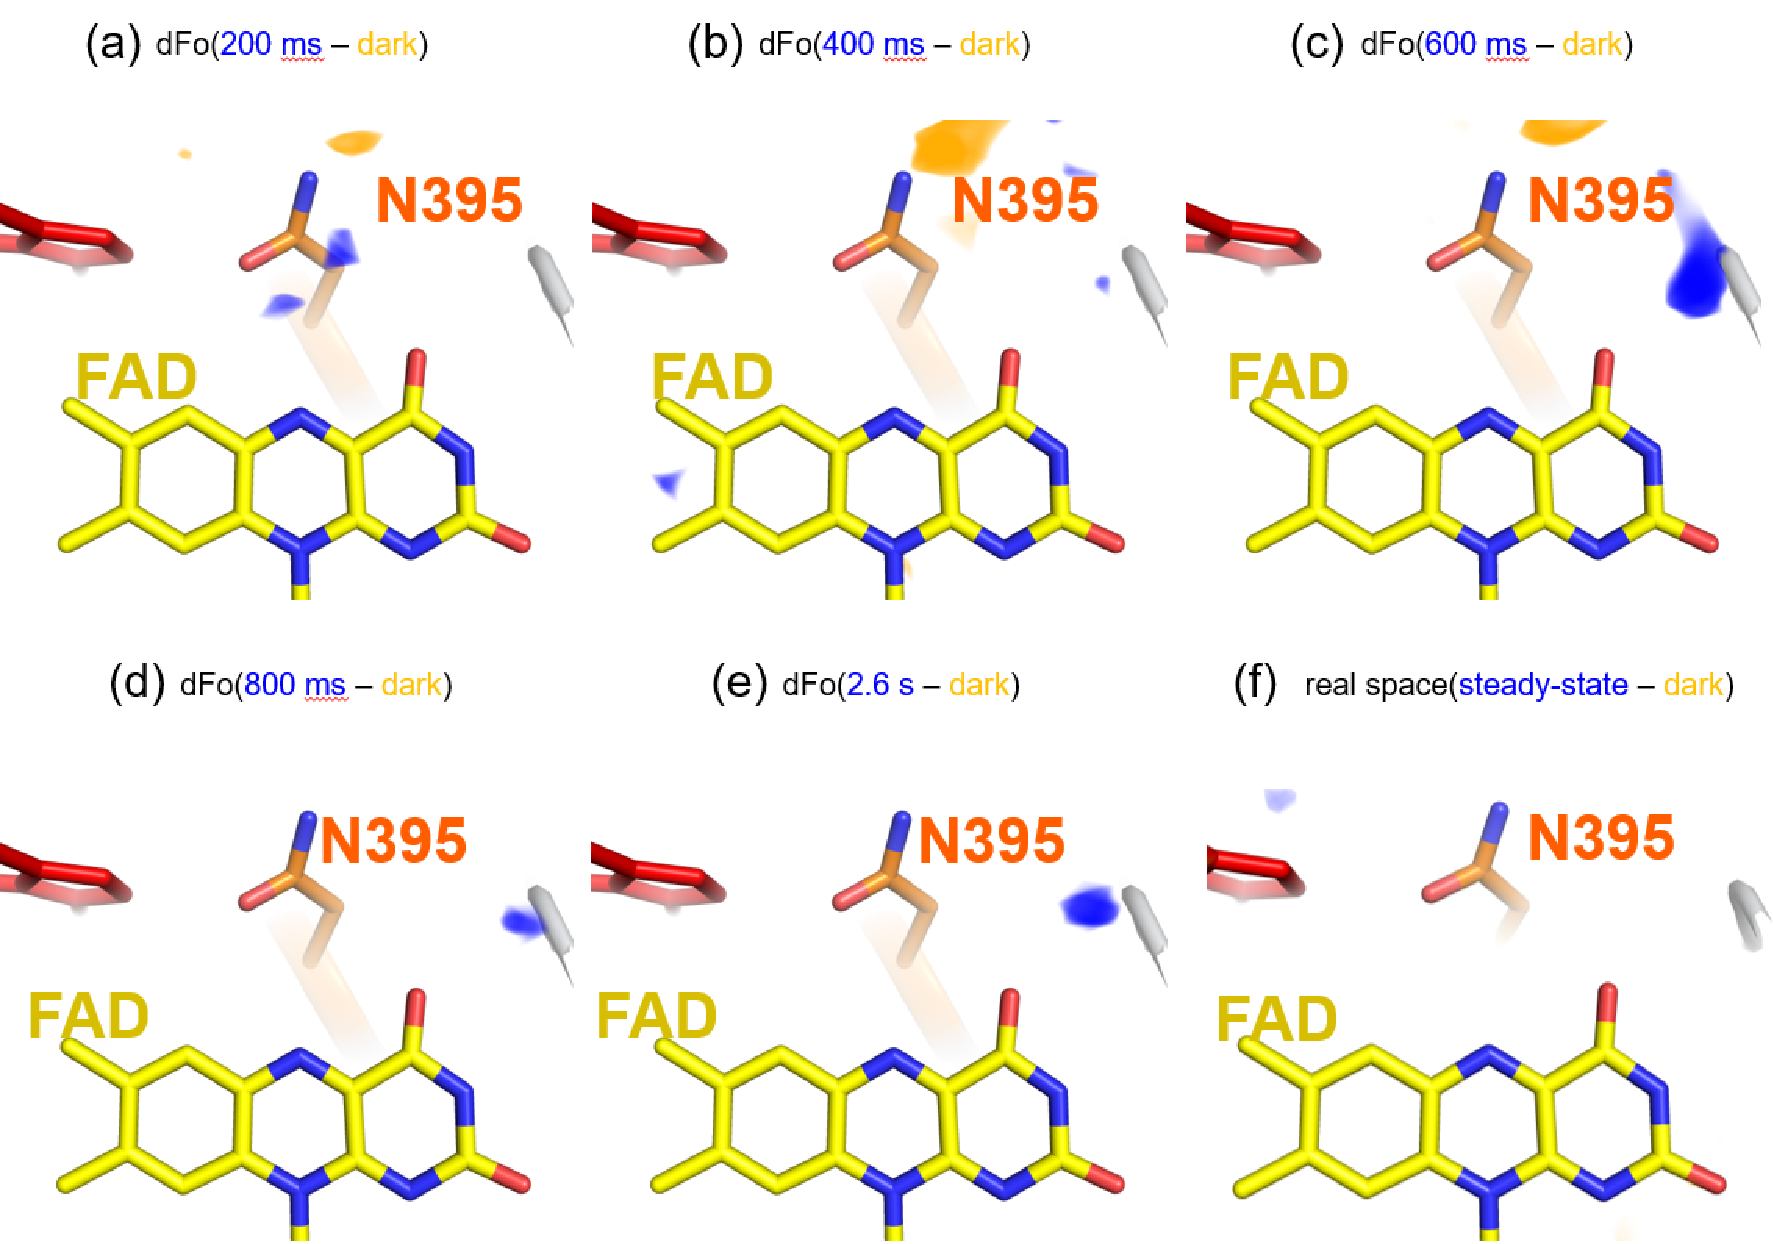
\includegraphics[width=\textwidth]{images/cracry/Supp_fig_FAD_CraCRY-TR-SOX_qFo.pdf}
  \hfill
  \caption{Decay of the FAD signal. TR-SOX data up to 3 s. Q weighted \parencite{bourgeoisNewProcessingTools1999, dezitterXtrapol8EnablesAutomatic2022} Isomorphous \(F_{obs}(time\ point) - F_{obs}(dark)\) maps from the TR-SOX experiment, centred on the FAD (resolution of these maps is much lower than that of the TR-SFX experiment, which decreases the signal levels, the maps have to be observed at 3.0 r.m.s.d. to be able to see relevant features). (a) 200 ms after the start of illumination,  positive difference density between N395 (orange) and the FAD (yellow) indicates that N395 has moved closer to the N5 atom of the isoalloxazine, but not rotated 90 \degree (b) 400 ms, (c) 600 ms, (d) 800 ms or (e) 2.5 s after the start of illumination, no density can be seen around neither the flavin nor N395. (f) real space electron density \(time\ point dark\) map centred on the flavin cofactor of CraCRY, with r.m.s.d signal also cut at 3.0 for comparison purposes. No density can be seed around the FAD or N395.}\label{supfig:TR-SOX_qFo_FAD}
\end{figure}


\section{Supplementary material Iron photoreduction in FutA}

\begin{figure}[H]
  \centering
  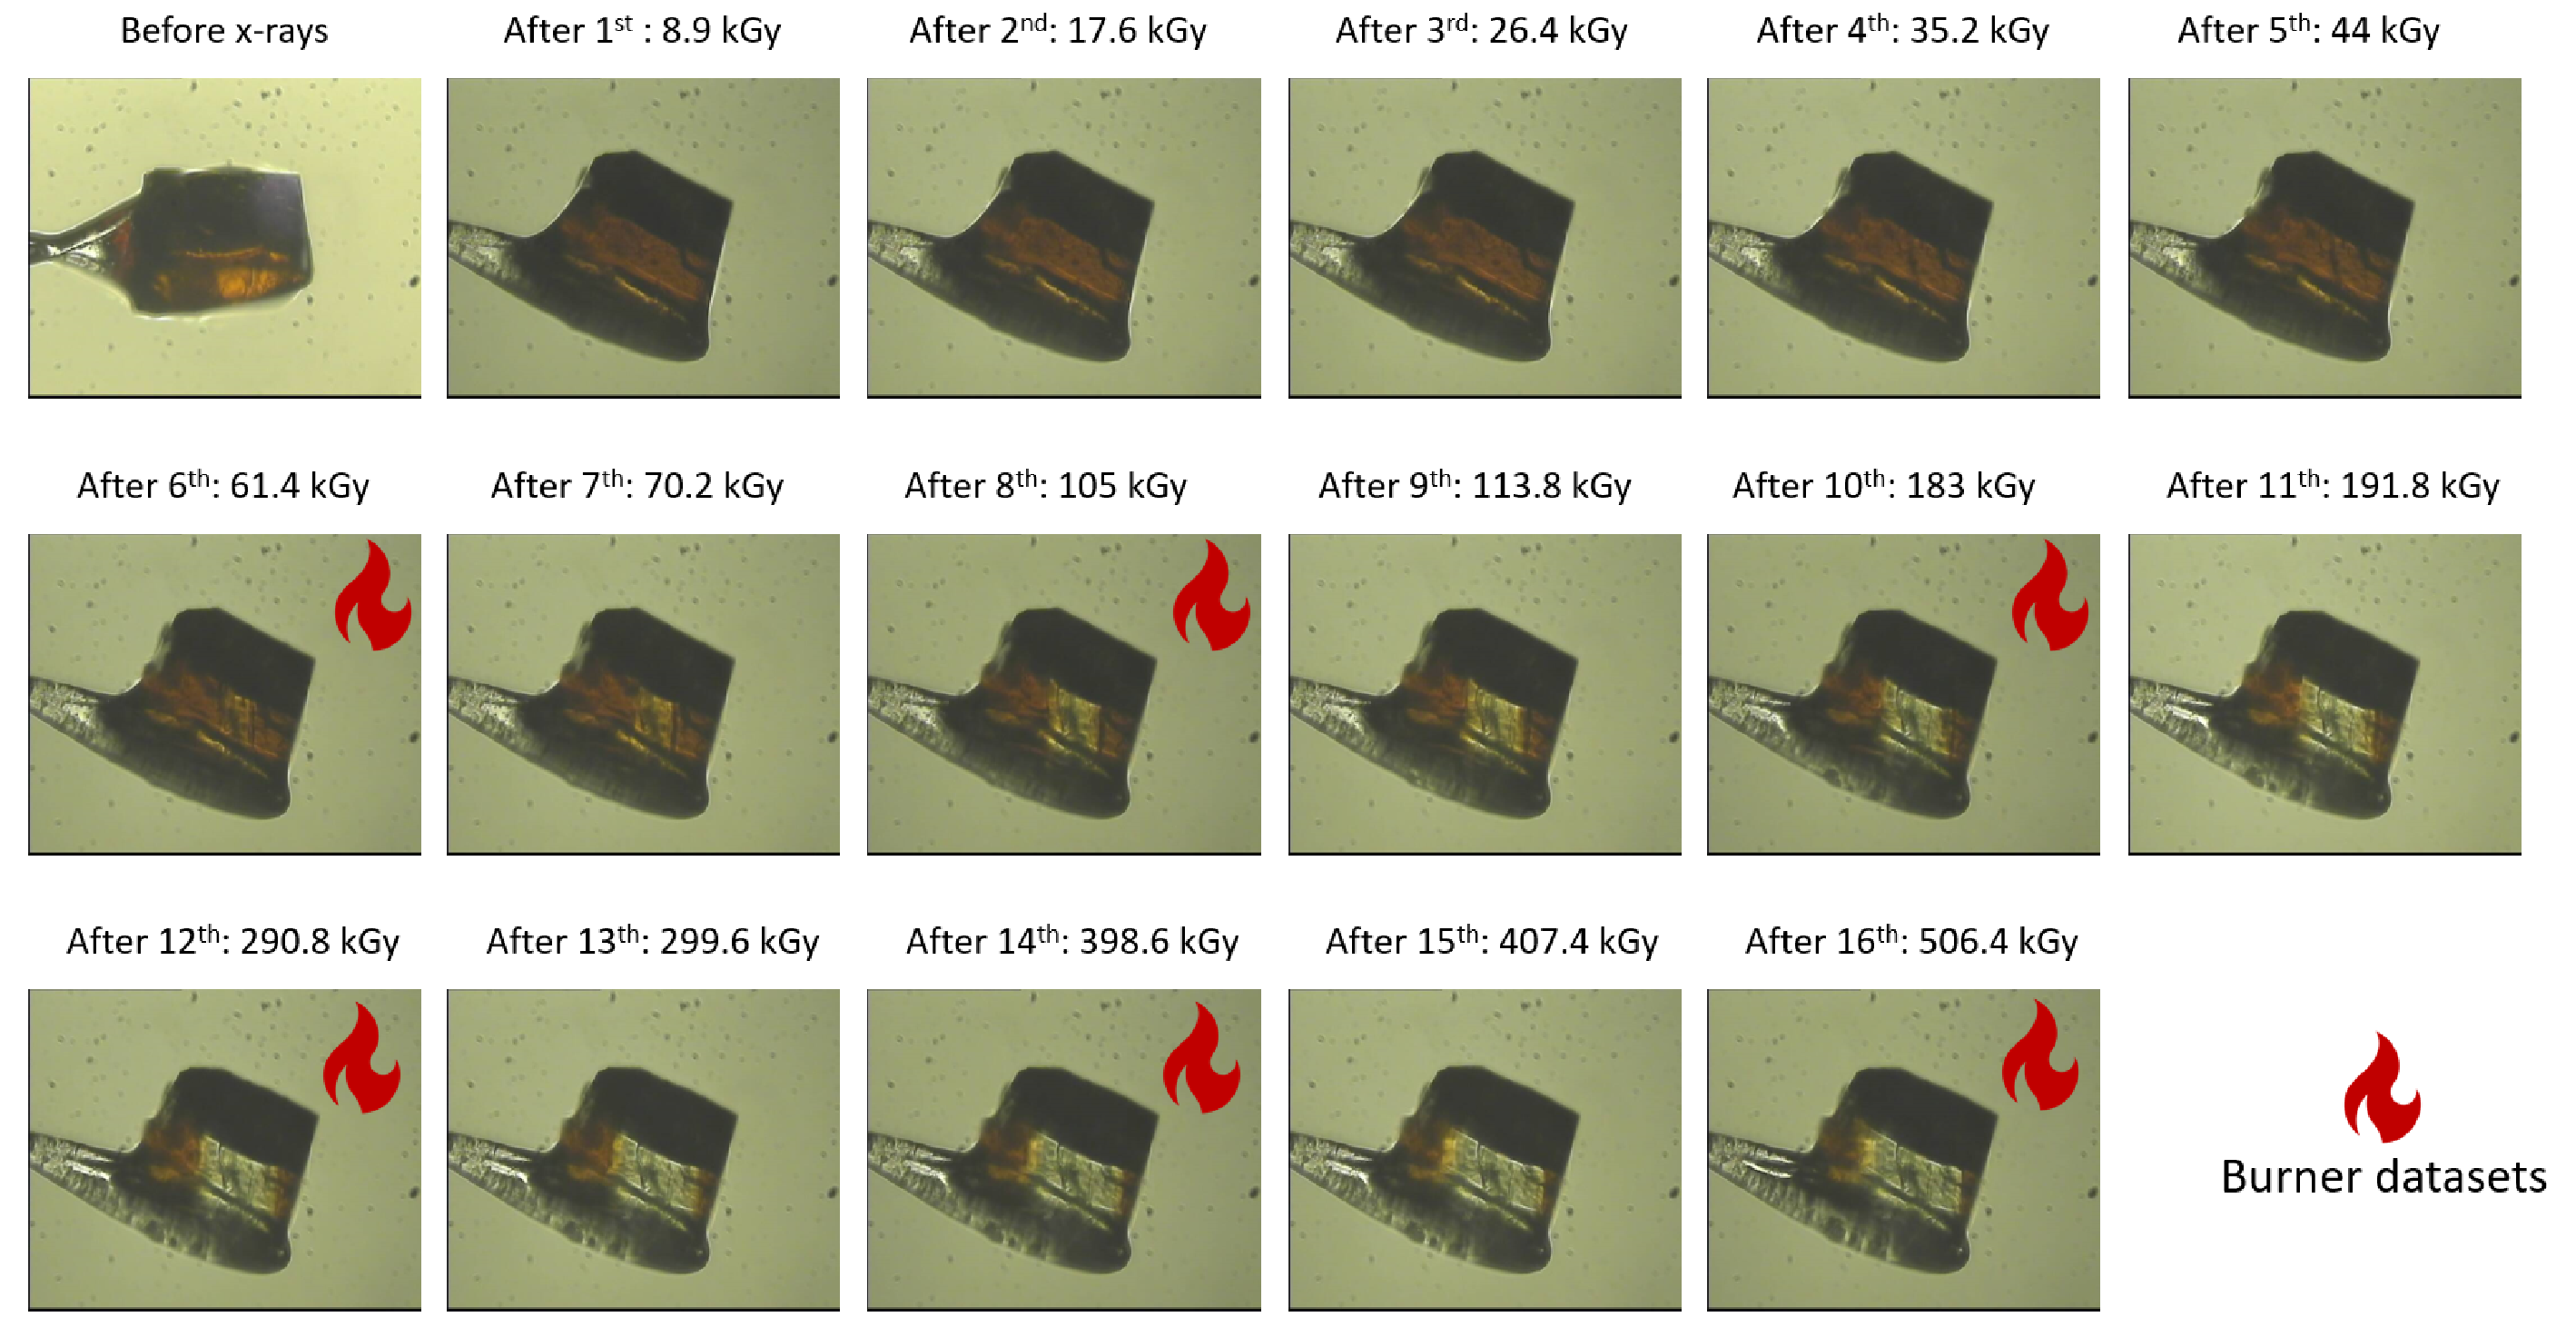
\includegraphics[width=\textwidth]{images/Spectroscopy/supp_FutA.pdf}
  \hfill
  \caption{Crystal of FutA, mounted on-axis of beamline BM07-FIP2, visibly losing its rust colour to turn transparent as diffraction datasets are collected (flux of \(3\times10^{10}\) photons / s). The red flame symbol represents so-called 'burner datasets' where transmission of the beamline was raised from 20 to 100 \% to reach a high dose faster. This is a reproduction of the initial data collection of FutA at room temperature, for documentation purposes.}\label{supfig:supfig_FutA}
\end{figure}


\section{New constructs of LOV2}\label{supchap:new_constructs}

The construct of LOV2 used in \cite{aumonierSlowProteinDynamics2022} and all studies carried out with LOV2 in this PhD has been obtained by mutating a construct of the miniSOG oxygen singulet producing protein \parencite{torraTailingMiniSOGStructural2019} into LOV2, but the C-terminal segment of this construct is not the physiological (long) linker between the LOV2 domain and its J\textalpha\, but rather a short helix-like segment, which does not fold in the same manner as the predicted structure of LOV2 in the full length protein (Fig. \ref{fig:PhotII_AF2} (a)). This prevented us from drawing any physiologically relevant conclusion from the photoadduct relaxation study. Constructs of the physiological sequence of LOV2 were ordered without (noJ\textalpha) with a truncated (half-J\textalpha) and with the full length (full-J\textalpha) J\textalpha\ helix. The constructs have been modeled using AlphaFold2 \parencite{jumperHighlyAccurateProtein2021, mirditaColabFoldMakingProtein2022} for illustration purposes, and are represented in Fig. \ref{supfig:newconstructs} (b). These constructs were inspired by the sturcture of the LOV2 domain from the phototropin II of \textit{Avena sativa} (2v1b, \cite{halavatyCTerminalFlankingRegions2007}). 

Of these constructs, only no-J\textalpha\ was crystallised, using a streak-seeding technique with cat-hair \parencite{bergforsSucceedingSeedingPractical2007} from crystals of the orginal LOV2 construct, using the same crystallisation condition as that described in Section \ref{sec:LOV2_methods}. It diffracted at a maximum resolution of 2 \AA at cryogenic temperature, on beamline id30b (ESRF, \cite{mccarthyID30BVersatileBeamline2018}). In this structure, with a resolution of 2 \AA, most of the C-terminus is not missing (yellow in Fig. \ref{supchap:new_constructs}), and the short segment still present point in a different direction to the C-terminus of the original LOV2 construct. In fact, SDS-page purification gels reveal that truncated vesions (lower molecular weights bands in Fig \ref{supfig:newconstructs} (c)) of the no-J\textalpha\ exist, hinting that the helix might have been cleaved at some point. The cleavage is clearly continuously happening during storage and purification as the truncated species are still visible after gel-filtration. This issue was also present for the half-J\textalpha\ and full-J\textalpha\ constructs, and no amounts of protease inhibitor ever solved it. All attempts at high throughput for the three constructs screening failed, very likely because the sample contained a mixture of cleaved and uncleaved protein. 

This is very likely because of the linker region between AtPhotIILOV2 and J\textalpha, which is much longer than that of the previously crystallised AsPhotIILOV2 \parencite{halavatyCTerminalFlankingRegions2007}, and therefore, more unstable. 

\begin{figure}[H] %bt!]
    \centering
    \noindent 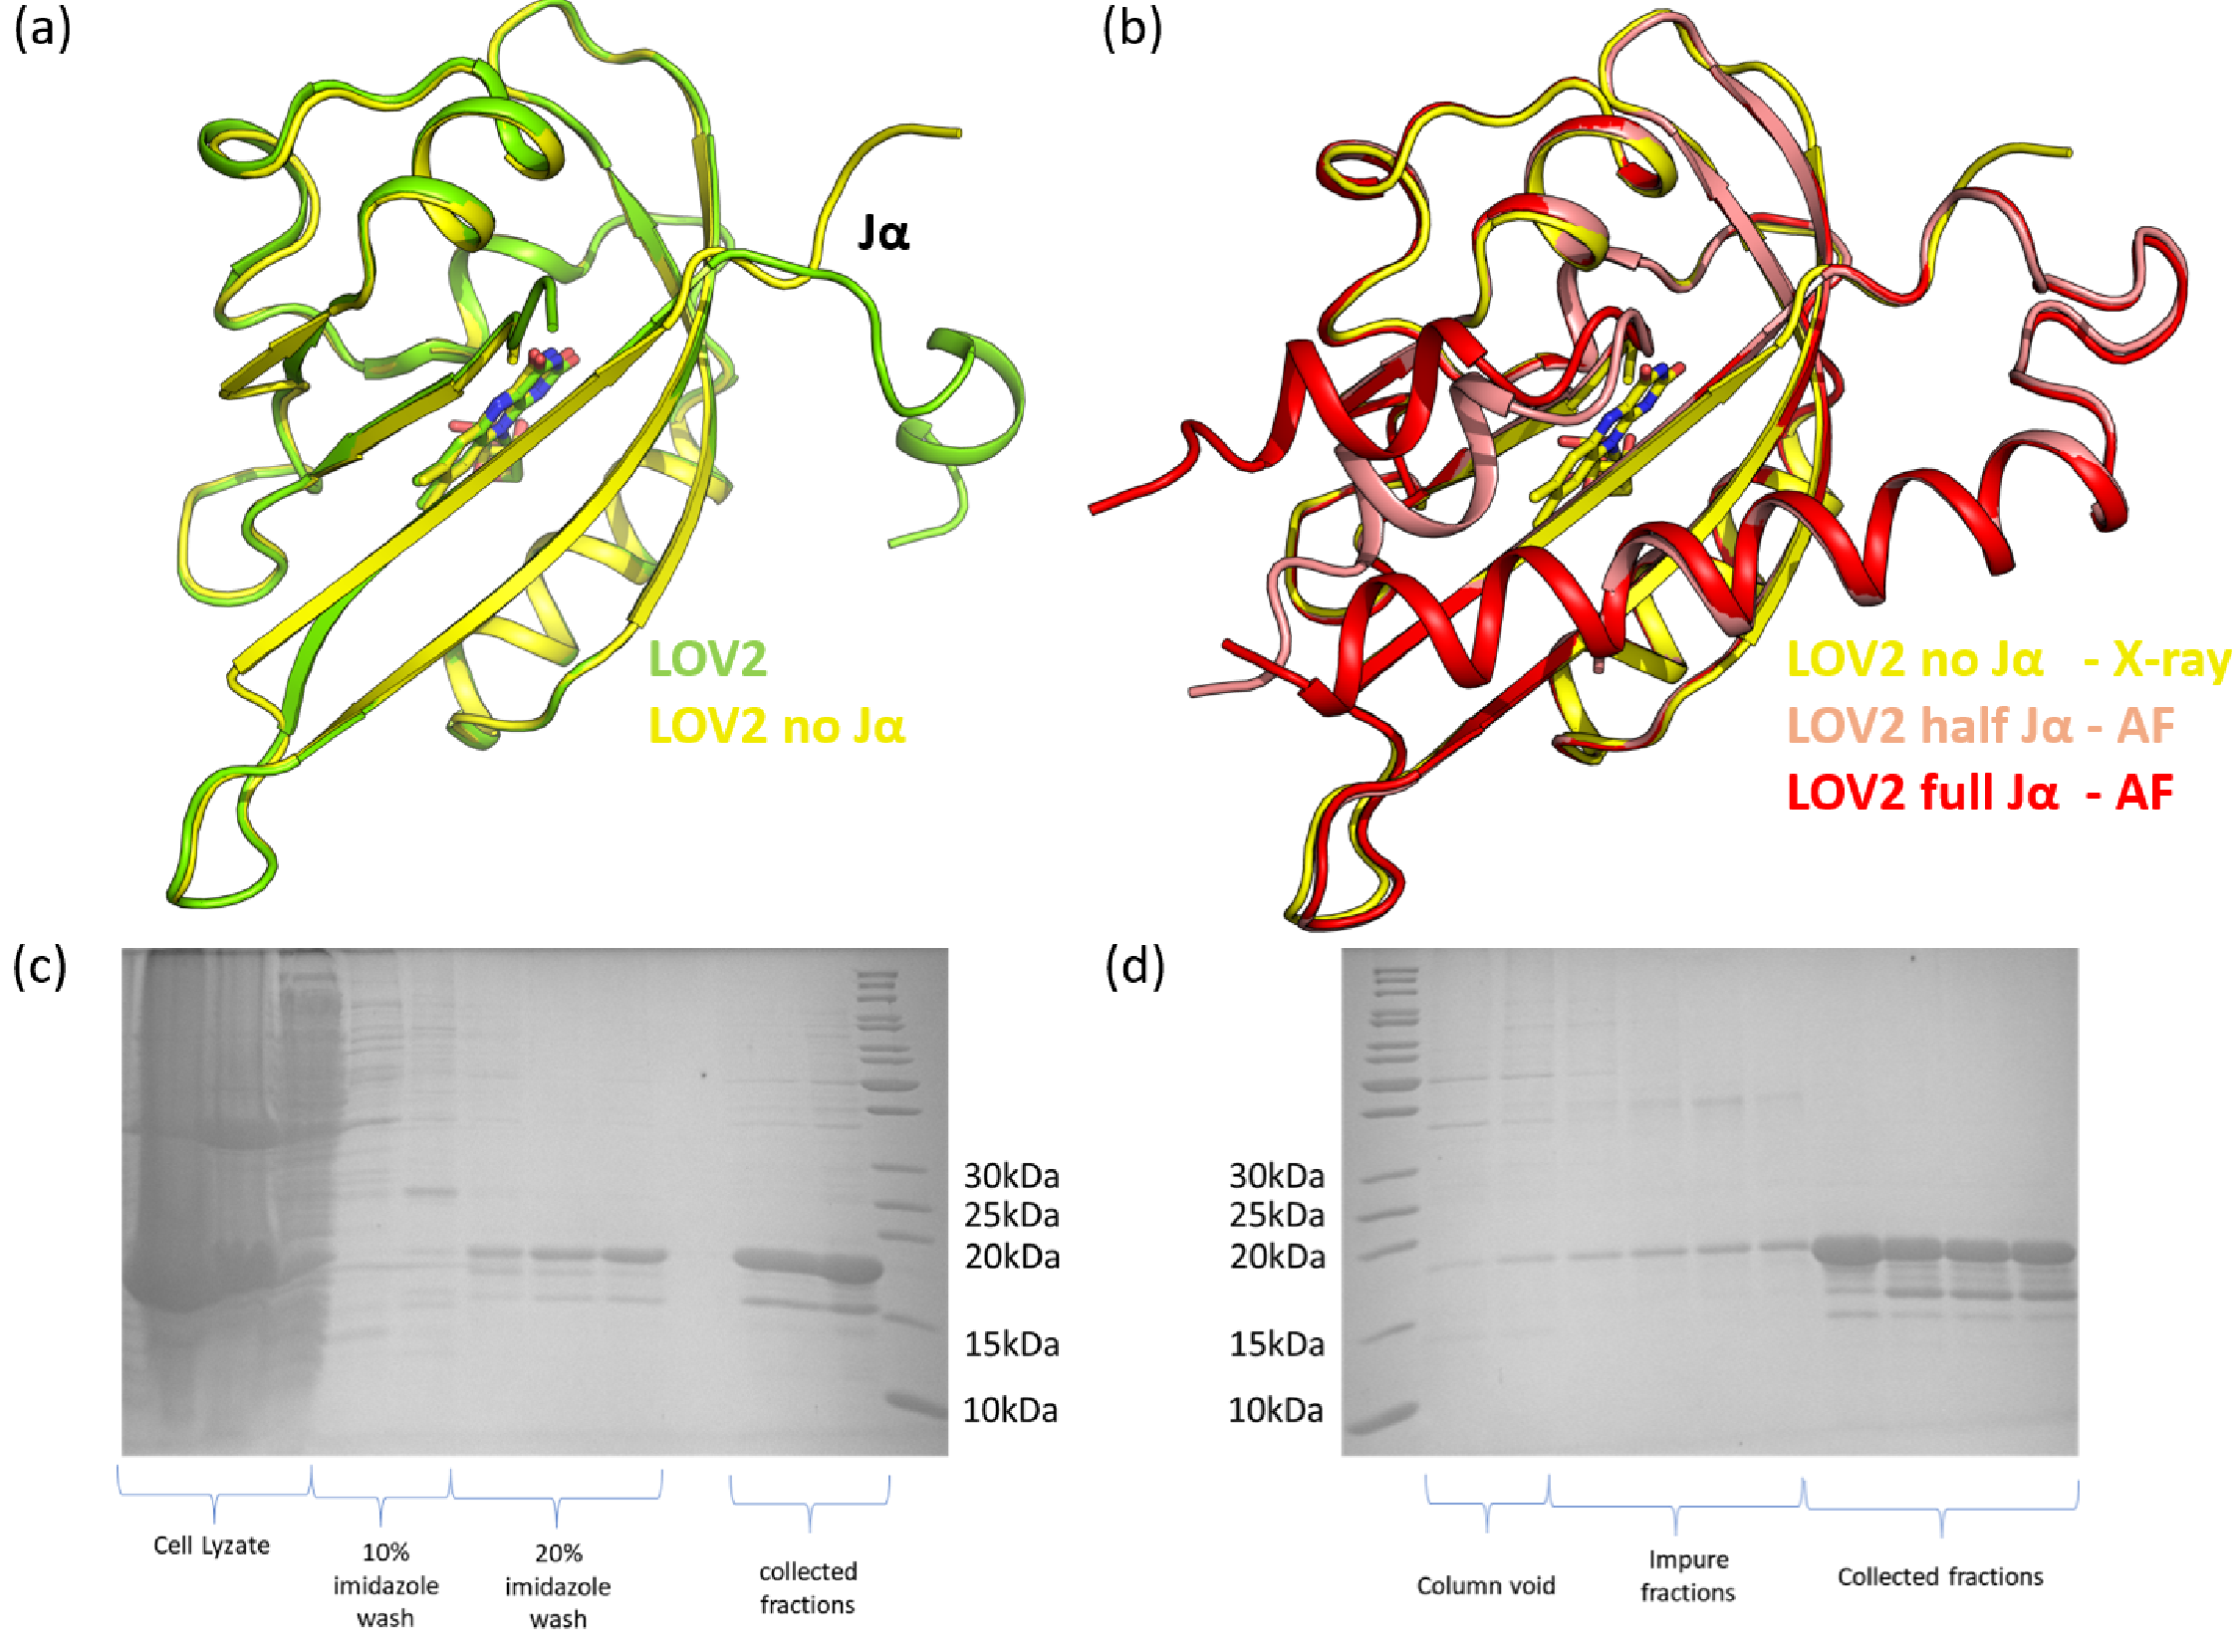
\includegraphics[width=\textwidth]{images/LOV2/new_constructs.pdf}
    \hfill
    \caption{New constructs of the AtPhotIILOV2. (a) Models from the X-ray structures of the construct used in \cite{aumonierSlowProteinDynamics2022}, coloured green, structure 6QQH, and no-J\textalpha\ constructs solved at cryogenic temperatures at 2.0 \AA resolution, coloured yellow. The main difference in the two models is in the fold of the C-terminus, which points upwards for the no-J\textalpha\ construct, and to the background for the LOV2 construct used in \cite{aumonierSlowProteinDynamics2022}. (b) Superposition of the X-ray structure of the no-J\textalpha\ construct (yellow) with the AlphaFold2 models of the half-J\textalpha\ (salmon) and full-J\textalpha\ (red) models. (c) SDS page gels from the purification of no-J\textalpha, for affinity and size-exclusion steps.}
    \label{supfig:newconstructs}
\end{figure}

\section{Supplementary material - \textit{ic}OS toolbox}

\subsection{Formats supported by the Toolbox}

The toolbox uses a custom file parser built around the csv reader function of PANDAS, python. The file formats presented in Table S1 have currently been tested, but any character-separated column-based file with a similar column layout should be compatible. We are committed to providing support for all ASCII file formats and welcome requests to extend the support to any specific layout. 
\begin{landscape}
\thispagestyle{empty} 
\begin{table}
\caption{Currently tested and supported formats }
\label{tab:formats_input}
    \begin{tabular}{>{\centering\arraybackslash}p{2cm}>{\centering\arraybackslash}p{2cm}>{\centering\arraybackslash}p{5cm}>{\centering\arraybackslash}p{1.7cm}>{\centering\arraybackslash}p{1cm}>{\centering\arraybackslash}p{1.5cm}>{\centering\arraybackslash}p{1cm}>{\centering\arraybackslash}p{1cm}>{\centering\arraybackslash}p{5cm}}
 \multicolumn{2}{c}{Spectrophotometer}& Column layout& Column separator & Decimal & Extension (.txt, .asc, .csv) & Header & Footer &Instrument producing the file\\
         manufacturer&  model& & & & & & & \\
         Ocean Optics & HR2000+ or QE65Pro - & Wavelength; Absorbance & Tab & . & .txt & 17 lines & 2 line & Main icOS lab setup - ESRF\\
         Ocean Optics & QE65 & Wavelength; Absorbance & Tab & . & .txt & 14 lines & 1 empty line & Online spectrophotometer BM07-FIP2 - ESRF\\
         Avantes & AvaSpec-ULS2048CL-EVO-RS-UA & Wavelength; Sample photon count; Dark reference photon count; Light reference photon count; Absorbance & ; & . & .txt & 8 &  & TR-icOS instrument – ESRF\\
         JASCO & FP-8500 & Wavelength; Absorbance & ; & , & .csv& 19 & 48 lines & Benchtop spectrophotometer\\
         ?? & ?? & Wavelength; Absorbance & Tab & . & .txt & 2 &  & Benchtop spectrophotometer\\
         Andor & Newton 970 EMCCD & Wavelength; Absorbance & Space & . & .asc &  & 34 lines & Online spectrophotometer I24 – Diamond Light Source\\
    \end{tabular}
\end{table}
\end{landscape}

\begin{table}
    \centering
\caption{Format of the file output of the toolbox}
\label{tab:formats_outputs}
    \begin{tabular}{cccc}
         Content of the file & Column layout & Column separator & Decimal separator\\
         Raw spectra & Wavelength; Absorbance & , & .\\
         Constant corrected spectra & Wavelength; Absorbance & , & .\\
         Scattering corrected spectra & Wavelength; Absorbance & , & .\\
    \end{tabular}
    
    
\end{table}

\subsection{Corrections}

\begin{figure}[H] %bt!]
    \centering
    \noindent 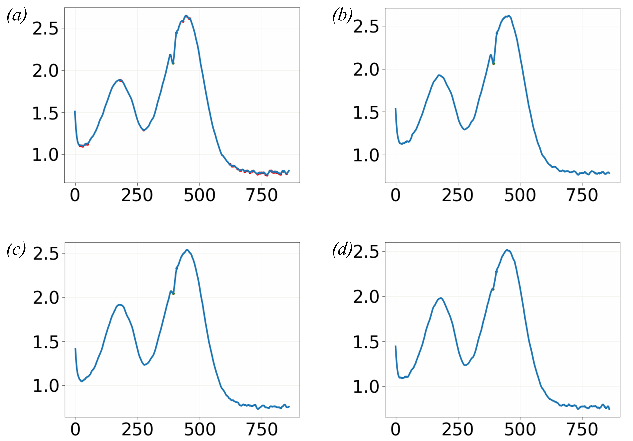
\includegraphics[width=\textwidth]{images/Spectroscopy/icOS_toolbox_FigS3.pdf}
    \hfill
    \caption{Laser dent-removal procedure for spectra of Bacteriorhodopsin at t=3 \textmu s (a), t=10 \textmu s (b), t=30 \textmu s (c), t=100 \textmu s (d). All dents are marked by red dots on the first spectrum, the laser dent - identified by the second derivative method - are marked by green dots. In the following spectra, only the main dent in the area of the previously detected laser dent. }
    \label{supfig:laserdent}
\end{figure}

\begin{figure}[H] %bt!]
    \centering
    \noindent 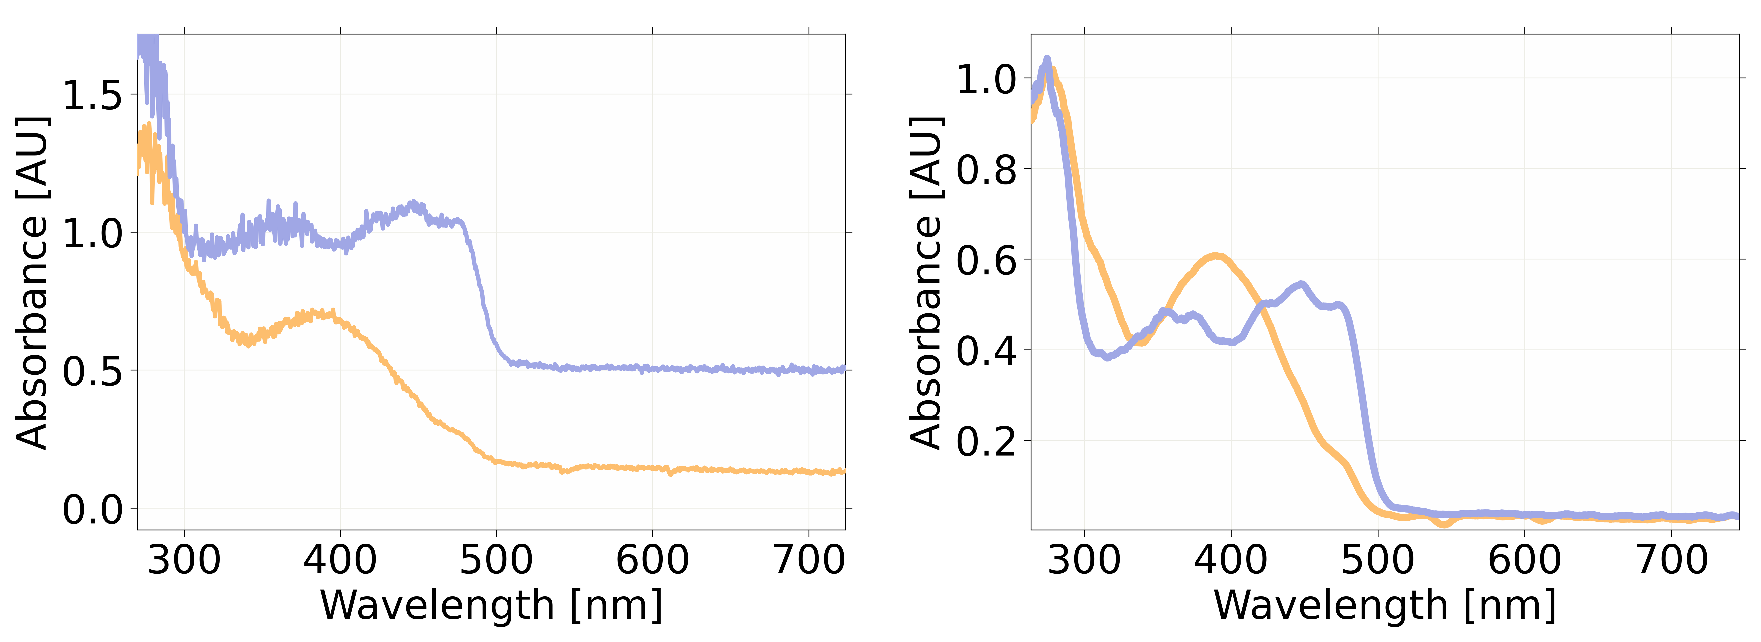
\includegraphics[width=\textwidth]{images/Spectroscopy/icOS_toolbox_Fig.S4.pdf}
    \hfill
    \caption{Scattering correction for plateaus in spectra of LOV2 from \cite{aumonierSlowProteinDynamics2022} in the dark (lavender) and photo-equilibrated (orange) spectra (a) Raw spectra (b) Corrected spectra}
    \label{supfig:plateau_correction}
\end{figure}

\begin{figure}[H] %bt!]
    \centering
    \noindent 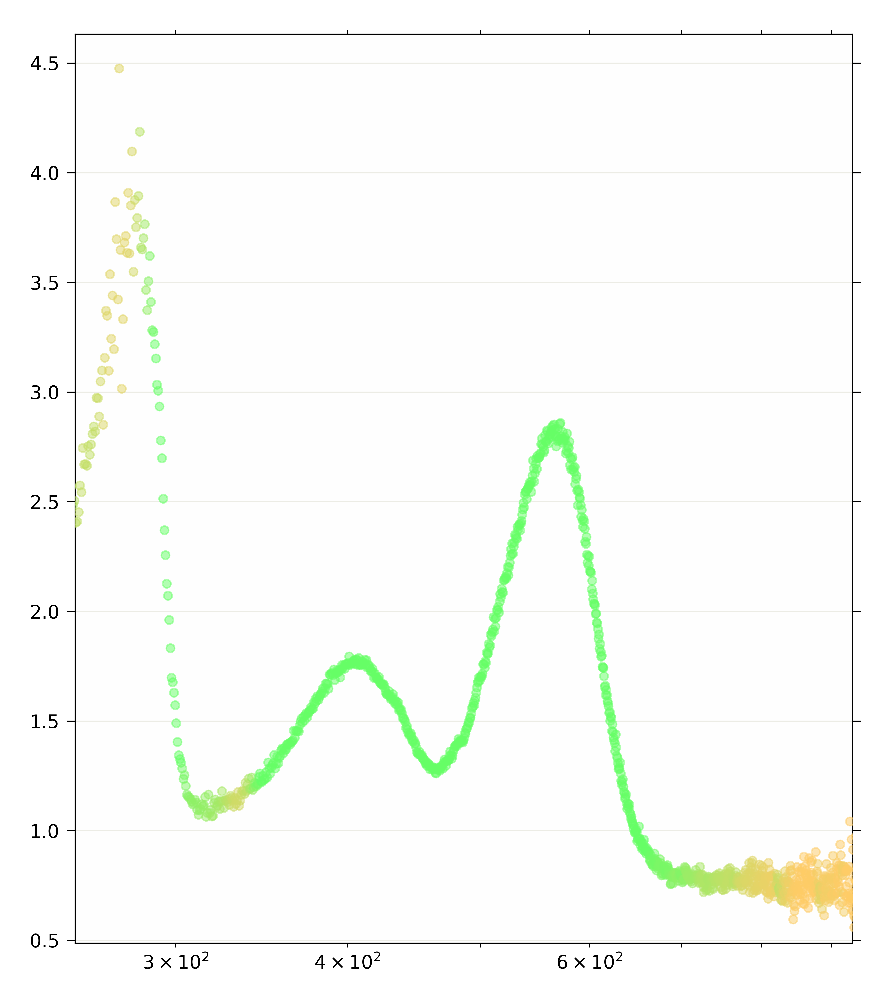
\includegraphics[width=\textwidth]{images/Spectroscopy/quality_TR-icOS.pdf}
    \hfill
    \caption{Quality score plot for a TR-icOS spectrum, green (high signal/noise) to orange (low signal/noise)}
    \label{supfig:quality}
\end{figure}


\section{DNA repair by the Class II photolyase of \textit{Methanosarcina mazei}\label{sec:paperMmCPDII}}
